%!TEX root = ./WTG.tex

\chapter{Irrfahrten und (elektrische) Netzwerke}
Thematisch scheinen diese beiden Begriffe nicht verwandt. Wir wollen sehen, dass dies nicht der Fall ist. Der Begriff \enquote{Irrfahrt} oder Markov-Kette sollte bekannt sein.
\section{Einführung Netzwerke}
\begin{definition}[Netzwerk] 
	\label{def:Netzwerk}
	\marginnote{Mit anderen Worten: Ein Netzwerk ist ein positiv gewichteter Graph.} 
	Ein Netzwerk $G = (V,E,c)$ ist ein Graph $\enb{V,E}$ mit entweder gerichteten oder ungerichteten Kanten, d.h.
	\begin{align}
		E \subseteq \set{\enb{x,y} \given x,y \in V} && \text{beziehungsweise} && E \subseteq \set{\set{x,y} \given x,y \in V},
	\end{align}
	zusammen mit einer Gewichtsfunktion $c:E \to \Real^+$.
\end{definition}

Ist nun $\enb{X_n}_n$ eine Irrfahrt auf $\enb{V,E}$ mit Übergangswahrscheinlichkeiten $P = \enb{p_{xy}}$, dann wollen wir daraus ein Netzwerk konstruieren. Dazu nehmen wir an, dass die Irrfahrt \emph{reversibel} bezüglich eines Maßes $\pi$ auf $V$ ist.
\begin{gather}
	\pi\enb{x}p_{xy} = \pi\enb{y} p_{yx}
\end{gather}
Dabei muss $\pi$ kein Wahrscheinlichkeitsmaß sein.

\begin{bemerkung}
	Das Maß $\pi$ ist stationär für die Markovkette.
\end{bemerkung}
\begin{beweis}
	Zu zeigen: $\pi \cdot \p = \pi$. 
	\begin{gather}
		\marginnote{$y\sim x:=$ alle $y$ die zu $x$ benachbart sind.}
		\pi\enb{x} = \pi\enb{x} \sum\limits_{y \sim x} p_{xy} = \sum\limits_{y \sim x} \pi(x)p_{xy} = \sum\limits_{y\sim x} \pi(y)p_{yx}.
	\end{gather}
\end{beweis}
Wählt man nun $c(x,y):=\pi(x)p_{xy}$ so gilt $c(x,y)=\pi(x)p_{xy} = \pi(y)p_{yx} =  c(y,x)$.
Das Kantengewicht ist also unabhängig von der Orientierung der Kante. Zusammenfassend haben wir nun festgestellt, dass eine reversible Irrfahrt bezüglich $\pi$ auf $(V,E)$ ein Netzwerk mit Kantengewicht $c(x,y) = \pi(x)\p_{xy} = c(y,x)$ induziert.

Umgekehrt existiert es zu einem gegebenen Netzwerk $(V,E,c)$ eine Irrfahrt auf $(V,E)$, mit $p_{xy} \approx c(x,y)$. Genauer: 
\begin{gather}	
p_{xy} = \frac{1}{\sum\limits_{z \sim x}} \cdot c(x,y) = \frac{c(x,y)}{\pi(x)}.
\end{gather}
Gilt $c(x,y) = c(y,x)$ für alle $x,y$, so ist die Irrfahrt bezüglich $\pi$ reversibel, denn 
\begin{gather}
	\pi(x)p_{xy} = c(x,y) = c(y,x) = \pi(y)p_{yx} 
\end{gather}

\begin{beispiel}[Gambler's Run]
	\label{bsp:GamblersRun}
	Sei $X_n$ eine Irrfahrt auf $\set{0, \dots, n}$ und	
	\begin{gather}
		\prop{X_n = i+1 \given X_{n-1} = i} = p = 1 - \prop{X_n = i-1 \given X_{n-1} = i}.
	\end{gather}
	Wie kommt man nun auf die Kantengewichte?
	\begin{gather}
		\prop{X_{n+1} = i+1 \given X_n = i} = \frac{c(i,i+1)}{c(i,i+1)+c(i,i-1)} = \frac{\enb{\frac{p}{q}}^i}{\enb{\frac{p}{q}}^i + \enb{\frac{p}{q}}^{i-1}} = \frac{\frac{p}{q}}{\frac{p}{q} +1} = p
	\end{gather}
	Sei nun $A,Z \subseteq V, A \cap Z = \emptyset$. Was ist nun $\prop{\tau_A < \tau_Z}[][x]?$ (Wobei $\tau_1$ die erste Treffzeit der Menge $A$ ist und $\p_x$ die Wahrscheinlichkeit, bei Start in $x$). Sei $F(x) = \prop{\tau_A < \tau_Z}[][x]$, dann ist $F|_A = 1$ und $F|_Z = 0$. Ist $x \notin A \cup Z$, dann ist $\set{x,y} \in E$ 
	\begin{equation}
		F(x) = \sum\limits_{y \sim x} p_{xy} F(y) = \frac{1}{\pi(x)} \sum\limits_{y \sim x} c(x,y)F(y) \tag{*} \label{eqn:GamblersRun}
	\end{equation}
	Im einfachsten Fall (Simple Random Walk) ist $c(x,y) = 1$ und $\pi(x) = \deg(x)$ \marginnote{$\deg(x)$ ist der Grad von $x$} und wir haben
	\begin{equation}
		F(x) = \frac{1}{\deg(x)} \sum\limits_{y \sim x} F(y),
	\end{equation}
	also ist $F(x)$ der Mittelwert all seiner Nachbarn. 
\end{beispiel}

\begin{definition}	
	Eine Funktion $F$, welche \eqref{eqn:GamblersRun} erfüllt, heißt harmonisch in $x$ bezüglich der Gewichte $c$. Ist $F$ harmonisch für alle $x \in V$ so heißt es nur harmonisch.
\end{definition}
Harmonische Funktionen erfüllen einige nützliche Prinzipien, Dazu sei für $W \subseteq V$
\begin{align}
	\delta W := \set{y \notin W \given \exists x \in W: y \sim x} && \overline{W} = W \cup \delta W
\end{align}
\begin{satz}[Maximumsprinzip]
	Sei $G(V,E,c)$ endlich oder unendlich und $H = (V(H),E(H),c)$ ein endliches zusammenhängendes Teilnetzwerk. Sei $f: V \to \RR$ harmonisch auf $H$. Falls dann gilt
	\begin{align}
		\max\limits_{x \in V(H)} f(x) = \sup\limits_G f
	\end{align}
	so gilt auf $V(H)$:
	\begin{align}
		f \equiv \sup f 
	\end{align}
\end{satz}
\begin{beweis}
	Sei $K := \set{f(x) = \sup f \given x \in V}$. Ist $x \in K \cap V(H)$, so gilt
	\begin{equation}
		\sup f = f(x) = \frac{1}{\pi(x)} \sum\limits_{y \sim x} c(x,y) f(y) \Rightarrow f(y) = f(x)
	\end{equation}
	für alle $y \sim x$. Das heißt, mit $x \in K$ sind auch alle $y \sim x$ in $K$. Da $V(H)$ endlich und zusammenhängend ist, kann man dies iterieren und kommt so bis $V(H) \cup \delta V(H) = \overline{V}(H)$.
\end{beweis}

\begin{korollar}[Eindeutigkeitsprinzip]
	\label{kor:Eindeutigkeitsprinzip}
	Sei $G = (V,E,c)$ beliebig, $W \subseteq V$ endlich. Falls $f,g: V \to \RR$ harmonisch auf $W$ sind, so folgt
	\begin{align}
		f|_{V\backslash W} = g|_{V\backslash W} \Rightarrow f = g
	\end{align}
\end{korollar}
\begin{beweis}
	Die Funktion $h = f - g$ ist harmonisch auf $W$ und $h=0$ auf $V\backslash W$. Wähle $x \in W$, sodass $h(x) > 0$ maximal ist. Wähle die Zusammenhangskomponente $W_0$ in der $x$ liegt. Dann ist $h \equiv h(x)$ auf $W_0 \cup \delta W_0$. Aber $\delta W \subseteq V \backslash W$ und dort ist $h(x) = 0 \lightning \Rightarrow h \leq 0$ überall. 
	
	Das gleiche stimmt für $\overline{h} = g-f \leq 0$.
\end{beweis}

\begin{korollar}
	\label{kor:1-7}
	Sei $V$ endlich, $A,Z \subseteq V, v \cap Z = \emptyset$. $G \colon V \to \Real$ erfüllen $G|_A = 1, G|_Z \equiv 0$ $G$ harmonisch auf $V \backslash (A \cap Z)$. Dann ist $G(x) = F(x) = \prop{\tau_A < \tau_Z}[][x]$
\end{korollar}
\begin{beweis}
	Folgt aus dem Eindeutigkeitsprinzip, wenn man $W = V\backslash (A \cap Z)$
\end{beweis}

\begin{satz}[Existenzprinzip]
	Sei $V$ endlich oder unendlich, $G = (V,E,c)$. Sei $W \nsubseteq V$ und $f_0 \colon V_0 \backslash W \to \Real$ beschränkt. Dann gibt es eine Funktion $f \colon V \to \Real$, sodass $f|_(v \backslash W) = f_0$ und $f|_W$ harmonisch.
\end{satz}

\begin{beweis}
	Starte die Netzwerk-Irrfahrt $(X_n)$, d.h. die deren Übergangswahrscheinlichkeiten durch $c(x,y)$ bestimmt sind. Sei $X$ die ZV, die angibt, wann $(X_n)$ die Menge $V \backslash W$ trifft, falls dies überhaupt der Fall ist. Sei
	\begin{gather}
		Y = 
		\begin{cases}
			f_0(X), & \text{falls} (X_n) \text{ die Menge } V \backslash W \text{ trifft } \\
			0, & \text{ sonst}
		\end{cases}
	\end{gather}
	Behauptung: $\EW{Y}$ ist eine harmonische Fortsetzung von $f_0$
\end{beweis}
\begin{uebung}
	Berechnen Sie im Gambler's Run die Wahrscheinlichkeit links oder rechts anzuschlagen, sowie die erwartete Treffzeit.
	\begin{figure}[htbp]
		\begin{minipage}{0.4\textwidth}
			\begin{tikzpicture}[scale = 0.8]
				\draw(0,0) to (7,0);
				\draw(0,3pt) to (0,-3pt) node[below] {0};
				\draw(7,3pt) to (7,-3pt) node[below] {n};
				\draw(3,3pt) to (3,-3pt);
				\draw [->, bend angle=45, bend right] (3,0) to (2,0);
				\draw [->, bend angle=45, bend left] (3,0) to (4,0);
				\draw node at(2.5,0.35) {$p-1$};
				\draw node at(3.5,0.35) {$p$};
			\end{tikzpicture}	
		\end{minipage} 
		\hfill
		\begin{minipage}{0.4\textwidth}
			\centering
			$p_X = p \cdot p_{X+1} + (1-p) p_{X-1} $
		\end{minipage}
	\end{figure}
\end{uebung}
Wir bertrachten jetzt ein Netzwerk als ein elektrisches Netzwerk, d.h. $c(x,y)$ sei die Leitfähigkeit und $\frac{1}{c(x,y)} = r(x,y)$ sei der Widerstand der Kante $(x,y)$. Wir legen in einem $a$ eine Spannung $v(a)$ an und leiten einen Strom $i$ durch das Netztwer, das in $Z \subseteq V$ abfließt ($v(z) = 0, \forall z \in Z$). Es gelten die klassischen Regeln der Elektrizitätslehre:

\begin{regel}[Ohmsches Gesetz]
	\label{regel:ohm}
	\begin{align}
		\forall x\sim y: v(x)-v(y) = i(x,y) \cdot r(x,y) = \frac{i(x,y)}{c(x,y)}
	\end{align}
\end{regel}

\begin{regel}[Kirchhoffsches Gesetz]
	\label{regel:kirch}
	\begin{align}
		\forall x \notin \set{a} \cup Z: \sum\limits_{y \sim x} i(x,y) = 0
	\end{align}
\end{regel}

Aus diesen Regeln lassen sich einige Konsequenzen ableiten:
\begin{itemize}
	\item da $c(x,y) = c(y,x) \Rightarrow i(x,y) = c(x,y)\big(v(x) -v(y)\big) = -c(x,y)\big(v(y)- v(x)\big) = - i(y,x)$
	\item da $c(x,y) > 0 \Rightarrow \Big({i(x,y) > 0 \Leftrightarrow v(x) > v(y)}\Big)$
	\item ist $x \notin A \cup Z$, so gilt nach \ref{regel:kirch} 
		\begin{align}
			0 = \sum\limits_{y \sim x} i(x,y) = \sum\limits_{y \sim x} \big[v(x)-v(y)\big]c(x,y)
		\end{align}
		Und wegen $c(x,y) = p_{xy} \cdot \pi(x)$, sowie im darauffolgenden Schritt $\sum\limits_{y \sim x} p_{xy} = 1$, folgt
		\begin{align}
			\Rightarrow \sum\limits_{y\sim x} v(y)c(x,y) = v(x)\pi(x) \sum\limits_{y \sim x} p_{xy} \\
			\Rightarrow v(x) = \frac{1}{\pi(x)} \sum\limits_{y \sim x} v(y) c(x,y)
		\end{align}
\end{itemize}
Also folgt aus \ref{regel:ohm} und \ref{regel:kirch}, dass $v$ harmonisch ist. Wenn also $V$ endlich ist, $V|_A = 1$ und $V|_Z \equiv 0$ ist, so folgt mit \ref{kor:1-7} $v(x) = \prop{\tau_A < \tau_Z}[][x]$

\begin{korollar}[Kirchhoffsche Maschenregel]
	Sei $x_1 \sim x_2 \sim \dots \sim x_n \sim x_1$ ein Kreis. Dann gilt 
	\begin{align}
		\sum\limits_{j=1}^{n}i(x_j,x_{j+1})r(x_j,x_{j+1}) = \sum\limits_{0}^{n}v(x_{j+1}) - v(x_j) = 0
	\end{align}
\end{korollar}

\section{Irrfahrten auf elektrischen Netzwerken}
Zunächst sei $G(V,E,c)$ nun immer ein endliches Netzwerk. Sei $a \in V$ und $Z \subseteq V$. Wir fragen uns nach der Wahrscheinlichkeit mit der Irrfahrt vom Startpunkt $a$ $Z$ zu erreichen, bevor wir wieder nach $a$ zurückkommen, also $\prop{a \to Z} = \prop{\tau_Z < \tau_{\set{a}}}[][a]$. Das wird insbesondere interessant, wenn $G$ unendlich, $G_n$ unendlich mit $G_n \uparrow G$ und  $Z = \delta G_n$ und $a=0$.

Dann fragt man sich offenbar nach der Wahrscheinlichkeit gegebenenfalls sehr weit von Ursprung entfernte Mengen $Z$ zu erreichen, bevor man $0$ wieder sieht. Das ist nichts anderes als Transienz. Wir wollen $\propE{a \to Z}[][a]$ studieren. Legen wir an $a$ eine Spannung $v(a)$ an und lassen $v(z) = 0, \forall z \in Z$ sein, dann ist $v$ auf $V \backslash(\set{a}\cup Z)$ harmonisch, aber auch $\propE{\tau_A < \tau_Z}[][x]$. Wegen des Eindeutigkeitsprinzips (\ref{kor:Eindeutigkeitsprinzip}) unterscheiden sich beide nun um $\frac{1}{v(a)}$, d.h. $\prop{\tau_a < \tau_Z}[][x] = \frac{v(x)}{v(a)}$. Also
\begin{align}
	\prop{a \to Z} = \sum\limits_{x}p_{ax} \Big(1-\prop{\tau_a \tau_Z}[][x] \Big) &= \sum\limits_{x}\frac{c(a,x)}{\pi(a)}\enb{1-\frac{v(x)}{v(a)}} \\
	&= \frac{1}{\pi(a)v(a)}\sum\limits_{x}c(a,x)\big(v(a)-v(x) \big) \\
	&= \frac{1}{\pi(a)v(a)}\sum\limits_{x}i(a,x)
\end{align}

\begin{align}
	\Rightarrow v(a) = \frac{\sum\limits_{x}i(a,x)}{\pi(a)\prop{a \to Z}}
\end{align}
Da $v(z) = 0$ auf $Z$, hat das Ganze wieder die Gestalt des Ohmschen Gesetztes \ref{regel:ohm}, wenn man den Nenner als Leitfähigkeit interpretiert. Tatsächlich heißt $\pi(a)\prop{a \to Z}$ die effektive Leitfähigkeit von $a$ nach $Z$ und wir schreiben
\begin{align} 
	\leit{a \leftrightarrow Z} = \mathcal{C}_{eff}  = \leit{a\leftrightarrow Z,G}
\end{align}
Den effektive Widerstand ist somit 
\begin{align}
	\frac{1}{\leit{a \to Z}} = R(a \leftrightarrow Z)
\end{align}
Offenbar ist $\prop{a\to Z} = \frac{\leit{a \leftrightarrow Z}}{\pi(a)}$. Das hilft allerdings nur, wenn $\leit{a \leftrightarrow Z}$ gut ausrechnen kann. 

Sei nun $X$ die Anzahl der Besuche von $X_n$ in $a$ bevor $X_n$ in $Z$ absorbiert wird. Wir betrachten zunächst den Start in $a$. Sei 
\begin{align}
	X \sim Geo(p) mit p= \prop{a \to Z} = \frac{\leit{a \leftrightarrow Z}}{\pi(a)} \\
	\EW{X} = \frac{\pi(a)}{\leit{a \leftrightarrow  Z}}
\end{align}
Legt man $v$ nun so an, dass $\sum i(a,x) = 1$ ein Einheitsstrom ist, dann gilt $\EW{X} = \pi(a)v(a)$.

Allgemeiner betrachten wir die erwartete Anzahl der BEsuche in $a$ bei Start in $a$ und Absorption auf $Z$.
\begin{definition}[Green's-Funktion]
	$\mathcal{G}(a,x) = \EW{\relax}_a \benb{\text{Besuche in $x$ vor Erreichen von Z}}$ heißt \emph{Green's-Funktion} für die Irrfahrt aus $G$ mit Absorption in $Z$.
\end{definition}

\begin{satz}
	Sei $G$ endlich, $v_i$ so, dass ein Einheitstrom in $a$ einfließt und $v(z) = 0, \forall z \in Z$. Dann gilt
	\begin{align}
		v(x) = \frac{\greens{a,x}}{\pi(x)}, \forall x \in V
	\end{align}
\end{satz}
\begin{beweis}
	Die rechte Seite erfüllt $\greens{a,a} = \pi(a) \cot v(a)$ und $\greens{a,z} = 0, z \in Z$, d.h. $\frac{\greens{a,x}}{\pi(x)}$ tut auf $\set{a} \cup Z$ das Gewünschte. Ist die rechte Seite auch harmonisch auf  $\enb{\set{a} \cup Z}^c$, so sind wir nach dem Gleichheitsprinzip fertig. Das ist eine Übung.
\end{beweis}
Heuristik: Strom ist eine Irrfahrt von $a$ nach $Z$ und $i(x,y)$ ist gerade die Netto--Anzahl der Überquerungen von $(x,y)$.

\begin{satz}
	Sei $(X_n)_n$ die Irrfahrt bei Start in $\set{a}$ und Absorption in $Z$ und $S_{xy} = $\enquote{Anzahl Überquerungen von $(x,y)$}. Dann gilt
	\begin{align}
		\EW{S_{xy}} = \greens{a,x}p_{xy} && \text{und} && \EW{S_{xy} - S_{yx}} =i(x,y) 
	\end{align}
\end{satz}
\begin{beweis}
	\begin{align}
		\EW{S_{xy}} = \sum\limits_{n=0}^{\infty} \mathds{1}_{\set{X_n=x,X_{n+1}=y}} &= \sum\limits_{n=0}^{\infty}\prop{X_n =x,X_{n+1} = y} \\
		&= \sum\limits_{n=0}^{\infty} \prop{X_n = x}p_{xy} \\
		&= p_{xy} \EW{\relax}\Big(\sum\limits_{n = 0}^{\infty} \mathds{1}_{\set{X_n = x}}\Big) \\
		&= p_{xy}\greens{a,x}
	\end{align}
	Und damit 
	\begin{align}
		\EW{S_{xy} - S_{yx}} = \greens{a,x}p_{xy} - \greens{a,x}p_{yx} = v(x) \underbrace{\pi(x)p_{xy}}_{\mathclap{c(x,y)}} - v(y) \underbrace{\pi(y)p_{xy}}_{\mathclap{c(y,x)=c(x,y)}} = i(x,y)
	\end{align}
\end{beweis}
\marginnote{Beginn Vorlesung 18.04.2016}
Wir wollen im Lauf dieser Sitzung den effektiven Widerstand nutzen, um Fragen der Rekurrenz und Transienz zu klären. Dazu benötigen wir ein unendliches Netzwerk $G = (V,E,c)$. Sei  nun $G_n$ eine gegen $G$ aufsteigende Folge endlicher Netzwerke, d.h. $G_n \subseteq G_{n+1}$ und $\bigcup G_n = G$. Sein $a \in G_n, \forall n$. Wir fragen uns nach $\prop{\text{\enquote{ich verlasse $G_n$, bevor ich $a$ wiedersehe}}}[][a]$.
Sei $Z_n = V \backslash V(G_n)$. Diese identifizieren wir mit einem Vertex $z_n$ in einem Netzwerk $G^W_n$. \marginnote{$V(G^W_n)  = V(G_n) \cup \set{z_n}$} Beim Identifizieren von $Z_n$ mit $z_n$ entstehen Schlaufen und Doppelkanten. Schlaufen lassen wir weg, Doppelkanten behalten wir. Die Folge von Ereignissen $\big(\set{a \to Z_n}\big)_n$ ist fallend. Also existiert $\lim \prop{a \to z_n}$. Die Irrfahrt ist transient, falls $\lim\limits_{n \to \infty} \prop{a \to z_n} > 0$. Dies ist genau dann wahr, wenn $\lim\limits_{n \to \infty} \leit{a \leftrightarrow z_n} > 0$.

\begin{satz}
	Die Irrfahrt auf $G$ ist genau dann transient, wenn zwischen $0$ und $\infty$ die effektive Leitfähigkeit  $\lim\limits_{n \to \infty} C(a \to z_n) > 0$ ist. 
\end{satz}

Um dies nützlich zu machen, benötigen wir eine Methode um $C(a \leftrightarrow z_n)$ zu berechnen. Die Idee des folgenden Kapitels ist es ein endliches Netzwerk immer weiter zu reduzieren, bis man die effektive Leitfähigkeit als Leitfähigkeiten ablösen kann.

\section{Reduktionsmethoden}
Wie lassen sich Netzwerke verkleinern?
\subsubsection*{Erstes Prinzip: Reihenschaltung}
Zwei Widerstände $r_1$ und $r_2$ in Reihe geschaltet verhalten sich wie ein Widerstand der Größe $r_1 + r_2$. Mit anderen Worten: in einem Netzwerk, das die Konfigurationen aus \autoref{fig:1-1} enthält, lassen sich die Zustände $(u_1,\omega)$ und $(\omega,u_2)$ ersetzen durch die Kante $(v_1,v_2)$  mit Widerstand $r_1+r_2$, ohne dass sich Ströme und Widerstände im restlichen Netzwerk ändern, siehe \autoref{fig:1-2}. Übung: Beweis. 

	\begin{figure}[b]
	\begin{subfigure}[t]{0.4\textwidth}
		\centering
		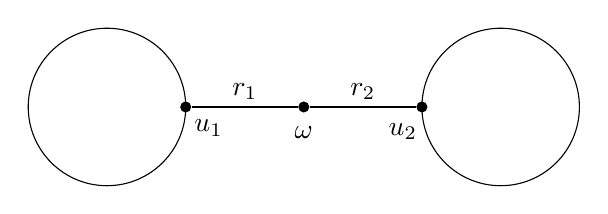
\begin{tikzpicture}[scale=1, every node/.style=fill,circle,minimum size=4pt,inner sep=0pt]
			\draw (0,0) circle (1);
			\draw (5,0) circle (1);
			\node[label={[label distance=3pt]320:{$u_1$}}] (u1) at (1,0) {};
			\node[label={[label distance=3pt]270:{$\omega$}}]  (omega) at (2.5,0) {};
			\node[label={[label distance=3pt]240:{$u_2$}}]  (u2) at (4,0) {};
			\draw (u1) -- (omega);
			\draw (omega) -- (u2);
			\node[fill=none] at (1.75,0.2) {$r_1$};
			\node[fill=none] at (3.25,0.2) {$r_2$};
		\end{tikzpicture}
		\subcaption{Verbindung der Teilnetzwerke über genau einen Knoten}
		\label{fig:1-1}
		\end{subfigure}
	\hfill
	\begin{subfigure}[t]{0.4\textwidth}
		\centering
			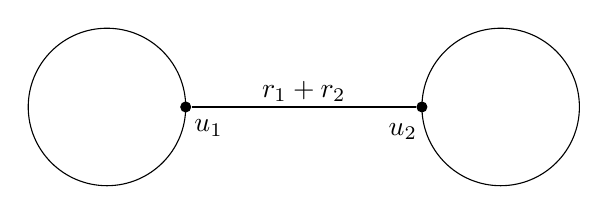
\begin{tikzpicture}[scale=1, every node/.style=fill,circle,minimum size=4pt,inner sep=0pt]
			\draw (0,0) circle (1);
			\draw (5,0) circle (1);
			\node[label={[label distance=3pt]320:{$u_1$}}] (u1) at (1,0) {};
			\node[label={[label distance=3pt]240:{$u_2$}}]  (u2) at (4,0) {};
			\draw (u1) -- (u2);
			\node[fill=none] at (2.5,0.2) {$r_1 + r_2$};
			\end{tikzpicture}	
		\subcaption{Ersetzen des Knotens durch Kante}
		\label{fig:1-2}
		\end{subfigure}
	\caption{Ersetzen von $\omega$}	
	\label{fig:1}
	\end{figure}


Wieso ist das nützlich?
\begin{beispiel}
	Sei $(X_n)_n$ die einfache Irrfahrt auf $\benb{0,n}$ mit Start in $k$. Frage: Was ist $\prop{\tau_0 < \tau_n}[][k]$? Wir wissen: Dies ist $v(k)$, wenn in $0$ eine Spannung $1$ und in $n$ eine Spannung $0$ anlegt.
	
	\begin{figure}[t]
		\begin{subfigure}[t]{0.4\textwidth}
			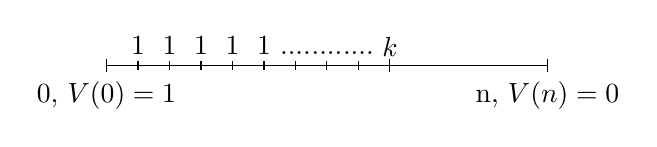
\begin{tikzpicture}[scale = 0.8]
				\draw(0,0) to (7,0);
				
				\draw(0,3pt) to (0,-3pt) node[below] {0, $V(0) = 1$};
				\draw(7,3pt) to (7,-3pt) node[below] {n, $V(n) = 0$};
				\foreach \x in {1,...,5}
				{
					\draw(0.5*\x,2pt) to (0.5*\x,-2pt) node[above=2pt] {1};
				}
				\foreach \x in {6,...,8}
				{
					\draw(0.5*\x,2pt) to (0.5*\x,-2pt) node[above=2pt] {....};
				}
				\draw(4.5,3pt) to (4.5,-3pt) node[above=2pt] {$k$};
			\end{tikzpicture}
			\subcaption{}
			\label{fig:1-3-1}
		\end{subfigure}
		\hfill
		\begin{subfigure}[t]{0.4\textwidth}
			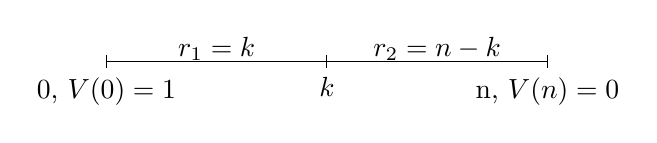
\begin{tikzpicture}[scale = 0.8]
			\draw(0,0) to (7,0);
			\draw(0,3pt) to (0,-3pt) node[below] {0, $V(0) = 1$};
			\draw(7,3pt) to (7,-3pt) node[below] {n, $V(n) = 0$};
			\draw(3.5,3pt) to (3.5,-3pt) node[below] {$k$};
			\node[fill=none] at (1.75,0.2) {$r_1 = k$};
			\node[fill=none] at (5.25,0.2) {$r_2 = n-k$};	
			\end{tikzpicture}
			\subcaption{}
			\label{fig:1-3-2}
		\end{subfigure}
		\caption{Zusammenführen mehrerer Kanten in Reihe}
	\end{figure}
	
	Nach dem Gesetz der Reihenschaltung kann man dieses Netzwerk (\ref{fig:1-3-1}) in folgendes Überführen(\ref{fig:1-3-2}) :
	\begin{gather}
		v(k) = \sum\limits_{y \sim k}\frac{c_{ky}}{\pi(k)}v_y = \frac{c_{k0}}{\pi(k)} \\
		\pi(k) = c_{k0} + c_{kn} = \frac{1}{k} + \frac{1}{k-n} = \frac{n}{k(n-k)} = \frac{n-k}{n}
	\end{gather}
	Allgemein gilt mit $q = 1-p$: $c(i,i+1) = \enb{\frac{p}{q}}^i$ und $v(i,i+1) = \enb{\frac{q}{p}}^i$.

	Dann kann man das Netzwerk (welches Analog zu \autoref{fig:1-3-2} ist) zusammenfassen mit 
	\begin{align}
		r_1 = \sum\limits_{i = 0}^{k-1}\enb{\frac{q}{p}}^i && r_1 = \sum\limits_{i = k}^{n-1}\enb{\frac{q}{p}}^i
	\end{align}

	Wieder ist 
	\begin{align}
		v_k = \frac{c_{k0}}{\pi(k)} && \pi(z) = \frac{\sum\limits_{i=0}^{n-1}\enb{\frac{q}{p}}^i}{\enb{\sum\limits_{i=0}^{k-1}\enb{\frac{q}{p}}^i} \enb{\sum\limits_{i=k}^{n-1} \enb{\frac{q}{p}}^i}} \\
	\end{align}
	\begin{align}
		\Rightarrow v_k = \frac{\sum\limits_{i=k}{n-1} \enb{\frac{q}{p}}^i}{\sum\limits_{i=0}^{n-1}\enb{\frac{q}{p}}^i} = \dots = \frac{\enb{\frac{p}{q}}^{n-k} -1}{\enb{\frac{p}{q}}^n-1}
 	\end{align}
\end{beispiel}
\subsubsection*{Zweites Prinzip: Parallelschaltung}
Man kann zwei parallele Leitungen mit Kapazitäten (Leitfähigkeiten) $c_1$ und $c_2$ durch eine einzige mit Leitfähigkeit $c_1+c_2$ ersetzen. Mit anderen Worten: In \autoref{fig:1-4} lässt sich die Doppelkante $(u_1,u_2)$ mit Leitfähigkeit $c_1$ und $c_2$ durch eine Kante $c_1+c_2$ ersetzen, ohne dass sich an den Spannungen und Strömen im Restnetzwerk etwas ändert. Übung: Beweis.

\begin{figure}
	\centering
	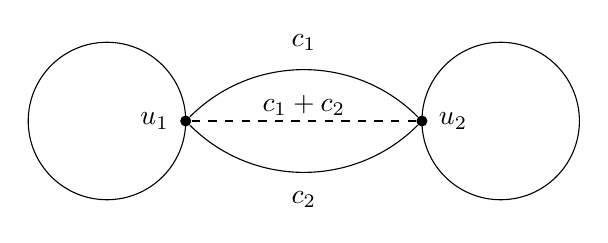
\begin{tikzpicture}[scale=1, every node/.style=fill,circle,minimum size=4pt,inner sep=0pt]
	\draw (0,0) circle (1);
	\draw (5,0) circle (1);
	\node[label={[label distance=3pt]180:{$u_1$}}] (u1) at (1,0) {};
	\node[label={[label distance=3pt]0:{$u_2$}}]  (u2) at (4,0) {};
	\draw [bend angle=45, bend right] (u1) to (u2);
	\draw [bend angle=45, bend left] (u1) to (u2);
	\node[fill=none] at (2.5,1) {$c_1$};
	\node[fill=none] at (2.5,-1) {$c_2$};
	\draw [dashed] (u1) to (u2);
	\node[fill=none] at (2.5,.2) {$c_1 + c_2$};
	\end{tikzpicture}	
	\caption{Zusammenlegen zweier parallel geschalteter Kanten.}
	\label{fig:1-4}
\end{figure}

\begin{beispiel} 
	Gefragt: $\propE{a \to z}$ im Netzwerk von \autoref{fig:1-5}. Durch die abgebildete Simplifizierung des Netwerkes erhalten wir direkt 
	\begin{align}
		\prop{a \to z} = \frac{\mathcal{C}(a \leftrightarrow z)}{i(a)} = \frac{\frac{7}{12}}{3} = \frac{7}{36}
	\end{align}
	%!TEX root = ../../WTG.tex

\begin{figure}
	\centering
	\subcaptionbox{Ausgangsnetzwerk}[0.49\textwidth]{
		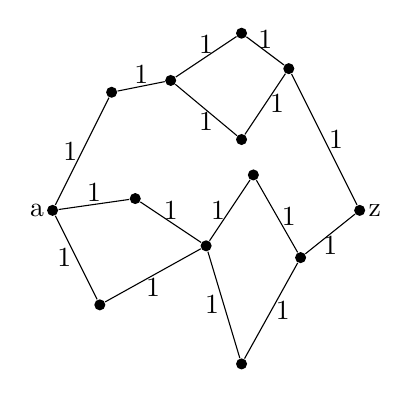
\begin{tikzpicture}[scale=1.5, every node/.style=fill,circle,minimum size=4pt,inner sep=0pt]
			\node [label=left:{a}] (a) at (0,0) {};
			\node (1) at (0.5,1) {};
			\node (2) at (1,1.1) {};
			\node (3) at (1.6,1.5) {};
			\node (4) at (1.6,0.6) {};
			\node (5) at (2,1.2) {};
			\node[label=right:{z}] (z) at (2.6,0) {}; 
			\node (6) at (0.7,0.1) {};
			\node (7) at (0.4,-0.8) {};
			\node (8) at (1.3,-0.3) {};
			\node (9) at (1.7,0.3) {};
			\node (10) at (1.6,-1.3) {};
			\node (11) at (2.1,-0.4) {};
			\draw (a) -- (1) node [midway, left, fill=none] {1};	
			\draw (1) -- (2) node [midway, above, fill=none] {1};	
			\draw (2) -- (3) node [midway, above, fill=none] {1};	
			\draw (2) -- (4) node [midway, below, fill=none] {1};
			\draw (4) -- (5) node [midway, right, fill=none] {1};		
			\draw (3) -- (5) node [midway, above, fill=none] {1};	
			\draw (5) -- (z) node [midway, right, fill=none] {1};	
			\draw (a) -- (6) node [midway, above, fill=none] {1};
			\draw (a) -- (7) node [midway, left, fill=none] {1};
			\draw (6) -- (8) node [midway, above, fill=none] {1};
			\draw (7) -- (8) node [midway, below, fill=none] {1};	
			\draw (8) -- (9) node [midway, left, fill=none] {1};	
			\draw (8) -- (10) node [midway, left, fill=none] {1};
			\draw (9) -- (11) node [midway, right, fill=none] {1};	
			\draw (10) -- (11) node [midway, right, fill=none] {1};	
			\draw (11) -- (z) node [midway, below, fill=none] {1};						
			%\draw (d) -- \node at (1,1) {} \node[fill=none,midway,label=above:{1}] {};
		\end{tikzpicture}
	}
	\hfill
	\subcaptionbox{Reihenschaltungen zusammengezogen}[0.49\textwidth]{
		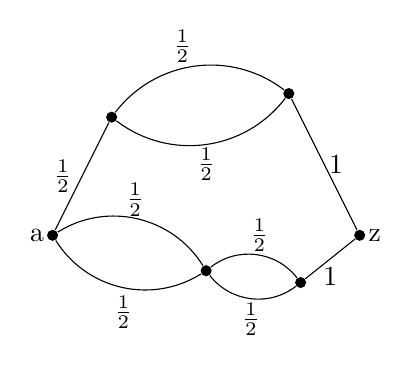
\begin{tikzpicture}[scale=1.5, every node/.style=fill,circle,minimum size=4pt,inner sep=0pt]
		\node [label=left:{a}] (a) at (0,0) {};
		\node (1) at (0.5,1) {};
		\node (2) at (2,1.2) {};
		\node[label=right:{z}] (z) at (2.6,0) {}; 
		\node (3) at (1.3,-0.3) {};
		\node (4) at (2.1,-0.4) {};
		
		\draw (a) -- (1) node [midway, left, fill=none] {$\frac{1}{2}$};
		\draw[bend angle=45,bend left] (1) to (2);
		\node [fill=none] at (1.1,1.6) {$\frac{1}{2}$};
		\draw[bend angle=45,bend right] (1) to (2);
		\node [fill=none] at(1.3,0.6) {$\frac{1}{2}$};
		\draw (2) -- (z) node [midway, right, fill=none] {$1$};
		\draw[bend angle=45,bend left] (a) to (3);
		\node [fill=none] at (0.7,0.3){$\frac{1}{2}$};
		\draw[bend angle=45,bend right] (a) to (3);
		\node [fill=none] at(0.6,-0.65) {$\frac{1}{2}$};	
		\draw[bend angle=45,bend left] (3) to (4);
		\node [fill=none] at (1.75,0) {$\frac{1}{2}$};
		\draw[bend angle=45,bend right] (3) to (4);
		\node [fill=none] at (1.68,-0.71) {$\frac{1}{2}$};	
		\draw (4) -- (z) node [midway, below=2pt, fill=none] {$1$};				
		%\draw (d) -- \node at (1,1) {} \node[fill=none,midway,label=above:{1}] {};
		\end{tikzpicture}
	}
	\hfill
	\subcaptionbox{Parallelschaltungen zusammengezogen}[0.30\textwidth]{
		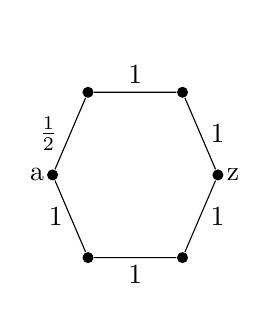
\begin{tikzpicture}[scale=1.5, every node/.style=fill,circle,minimum size=4pt,inner sep=0pt]
			\node [label=left:{a}] (a) at (0,0) {};
			\node (1) at (0.3,0.7) {};
			\node (2) at (1.1,0.7) {};
			\node[label=right:{z}] (z) at (1.4,0) {}; 
			\node (3) at (0.3,-0.7) {};
			\node (4) at (1.1,-0.7) {};
			\draw (a) -- (1) node [midway, left=1pt, fill=none] {$\frac{1}{2}$};
			\draw (1) -- (2) node [midway, above=2pt, fill=none] {$1$};
			\draw (2) -- (z) node [midway, right=2pt, fill=none] {$1$};
			\draw (a) -- (3) node [midway, left=1pt, fill=none] {$1$};
			\draw (3) -- (4) node [midway, below=2pt, fill=none] {$1$};
			\draw (4) -- (z) node [midway, right=2pt, fill=none] {$1$};
			\node[fill=none] at (0,-0.8) {}; 
			\node[fill=none] at (0,1.2) {};	
		\end{tikzpicture}
	}
	\hfill
	\subcaptionbox{Reihenschaltungen erneut zusammengezogen}[0.30\textwidth]{
		\begin{tikzpicture}[scale=1.5, every node/.style=fill,circle,minimum size=4pt,inner sep=0pt]
			\node [label=left:{a}] (a) at (0,0) {};
			\node[label=right:{z}] (z) at (1.4,0) {}; 
			\draw[bend angle=45,bend right] (a) to (z);
			\node [fill=none] at (0.7,0.5) {$\frac{1}{4}$};
			\draw[bend angle=45,bend left] (a) to (z);
			\node [fill=none] at (0.7,-0.5) {$\frac{1}{3}$};
			\node[fill=none] at (0,-0.8) {}; 
			\node[fill=none] at (0,1.2) {};
		\end{tikzpicture}
	}
	\hfill
	\subcaptionbox{Parallelschaltungen erneut zusammengezogen}[0.30\textwidth]{
		\begin{tikzpicture}[scale=1.5, every node/.style=fill,circle,minimum size=4pt,inner sep=0pt]
		\node [label=left:{a}] (a) at (0,0) {};
		\node[label=right:{z}] (z) at (1.4,0) {}; 
		\node[fill=none] at (0,-0.8) {}; 
		\node[fill=none] at (0,1.2) {};
		\draw (a) to (z);
		\node [fill=none] at (0.7,0.2) {$\frac{7}{12}$};
		\end{tikzpicture}	
	}
	\caption{Schritt für Schritt Simplifizierung eines Netzwerks}
	\label{fig:1-5}
\end{figure}
\end{beispiel}


\begin{beispiel}
	Gesucht $\prop{a \to z}$ im Netzwerk von \autoref{fig:1-6}. Hier wenden wir ein \enquote{Physikerargument} an:
	Die Situation von $b$ und $c$ ist vollkommen identisch, daher gilt $v(b) = v(c)$ und somit $i(b,c) = 0$. Also kann man die Kante, welche die beiden verbindet auch einfach weglassen. Danach vereinfacht man das Netzwerk schrittweise analog zum vorigen Beispiel und erhält so
	\begin{align}
		\mathcal{C}(a \leftrightarrow z) = \frac{2}{3} \Rightarrow \prop{a \rightarrow z} = \frac{\frac{2}{3}}{2}= \frac{1}{3}
	\end{align}
	Spätestens wenn aber die an $b$ und $c$ angrenzenden Kanten unterschiedliches Gewicht haben wird das Argument allerdings problematisch.
	\begin{figure}
		\centering
		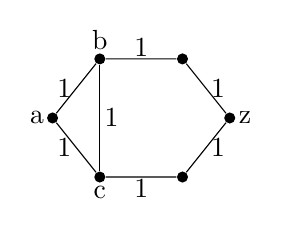
\begin{tikzpicture}[scale=1.5, every node/.style=fill,circle,minimum size=4pt,inner sep=0pt]
		
			\node [label=left:{a}] (a) at (0,0) {};
			\node [label=above:{b}] (1) at (0.4,0.5) {};
			\node (2) at (1.1,0.5) {};
			\node [label=below:{c}](3) at (0.4,-0.5) {};
			\node (4) at (1.1,-0.5) {};
			\node[label=right:{z}] (z) at (1.5,0) {}; 
			
			\draw (a) -- (1) node [midway, left, fill=none] {1};	
			\draw (1) -- (2) node [midway, above, fill=none] {1};	
			\draw (2) -- (z) node [midway, right, fill=none] {1};	
			\draw (a) -- (3) node [midway, left, fill=none] {1};
			\draw (3) -- (4) node [midway, below, fill=none] {1};	
			\draw (4) -- (z) node [midway, right, fill=none] {1};	
			\draw (1) -- (3) node [midway, right, fill=none] {1};
			
		\end{tikzpicture}
		\caption{Ausgangsnetzwerk für \enquote{Physikertrick}}
		\label{fig:1-6}
	\end{figure}
\end{beispiel}

\subsubsection*{Drittes Prinzip: Y--$\Delta$--Prinzip}
Auch Stein--Dreieck--Prinzip genannt. Netzwerke in denen man eine der Konfigurationen aus \autoref{fig:1-7} durch die andere ersetzt, sind äquivalent, falls 

\begin{figure}
	\centering
	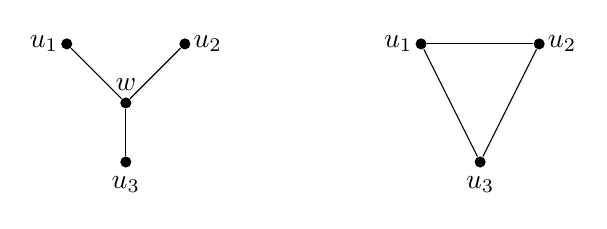
\begin{tikzpicture}[scale=1.5, every node/.style=fill,circle,minimum size=4pt,inner sep=0pt]
		\node [label=left:{$u_1$}] (u1) at (-0.5,0.5) {};
		\node [label=right:{$u_2$}] (u2) at (0.5,0.5) {};
		\node [label=below:{$u_3$}] (u3) at (0,-0.5) {};
		\node [label=above:{$w$}] (w) at (0,0) {};
		
		\node [label=left:{$u_1$}] (u1d) at (2.5,0.5) {};
		\node [label=right:{$u_2$}] (u2d) at (3.5,0.5) {};
		\node [label=below:{$u_3$}] (u3d) at (3,-0.5) {};
		
		\draw (u1) -- (w);
		\draw (u2) -- (w);
		\draw (u3) -- (w);
		\draw (u1d) -- (u2d);
		\draw (u2d) -- (u3d);
		\draw (u3d) -- (u1d);		 
	\end{tikzpicture}
	\caption{Äquivalente Konfigurationen}
	\label{fig:1-7}
\end{figure}


\begin{align}
	c(w, u_i) \cdot c(u_{i-1},u_{i+1}) = \gamma, \quad \forall i\ \text{mod}\ 3 &&
	\text{mit }\quad \gamma  = \frac{\prod_{i} c(w,u_i)}{\sum_{i}c(w,u_i)}
\end{align}
\subsubsection*{Viertes Prinzip (trivial):}
Man kann Knoten von Grad 1 hinzufügen oder entfernen. Selbiges Gilt für Schlaufen.

\marginnote{Beginn Vorlesung 21.04.2016}
Bislang haben wir gesehen, dass sich wichtige Fragen über Irrfahrten auf \enquote{elektrische Fragen} zurückführen lassen. Trefferwahrscheinlichkeiten entsprechen z.B. Spannungen, Durchquerungswahrscheinlichkeiten effektiven Kapazitäten usw. 
Durch Reduktion der Netzwerke lassen sich solche Größen auch berechnen. 

Heute wollen wir eine weitere Größe kennenlernen, die bei der Beantwortung von Fragen über Irrfahrten hilft.

\section{Energie}
\label{chap:Energie}
Sei zunächst $G = \enb{V,E,c}$ ein endliches Netzwerk.
\begin{definition}
	Sei $l^2\enb{V}$ die Menge aller Funktionen $F: V \to \RR$. $l^2(V)$ sei versehen mit dem üblichen Skalarprodukt 
	\begin{gather}
	\sprod{f,g} := \sum\limits_{v \in V} f(v)g(v), \Norm{f}^2 = \sprod{f,f}
	\end{gather}	
\end{definition}
\begin{definition}
	Sei $l^2(E)$ die Menge aller antisymmetrischen Funktionen 
	\begin{gather}
	\Theta = E \to \Real \text{ mit } \Theta(-e) = -\Theta(e)
	\end{gather}
	mit Skalarprodukt 
	\begin{gather}
	\sprod{\Theta,\Theta'} = \frac{1}{2}\sum\limits_{e \in E} \Theta(e) \Theta'(e) = \sum\limits_{e \in E_{1/2}} \Theta(e)\Theta'(e)
	\end{gather}
	wobei $E_{1/2}$ eine Teilmenge von $E$, die von jedem Paar $(e,-e), e \in E$ genau einen Vertreter enthält.
\end{definition}

\begin{definition}
	Sei $d:l^2(V) \to l^2(E)$ der \emph{Co-Rand-Operator}, definiert als
	\begin{gather}
	(df)(e) =  f(e^-) - f(e^+) \text{ wobei } e= (e^-,e^+)
	\end{gather}
	Weiter sei $d^*: l^2(E) \to l^2(V)$ der Rand Operator, definiert als
	\begin{gather}
	(d^*\Theta)(x) = \sum\limits_{e:e^-=x} \Theta(e)
	\end{gather}
\end{definition}
\begin{uebung}
	$\forall f \in l^2(V), \forall \Theta \in l^2_-(E)gilt$
	\begin{gather}
	\sprod{df,\Theta}_{l^2_-E} = \sprod{f,d^*\Theta}_{l^2(V)}
	\end{gather}
	Man kann Ohm und Kirchhoff mittels $d$ und $d^*$ elegant aufschreiben.
	\begin{itemize}
		\item Ohm: $dv = ir$, d.h. $\forall \ c \in E$ gilt $(dv)(e) = i(e) \cdot r(e)$.
		\item Kirchhoff: Für alle $x$, die nicht an einer Spannungsquelle liegen, gilt $(d^*i)(x)= 0$.
	\end{itemize}
\end{uebung}
Wir wollen nun Flüsse auf Netzwerken studieren. Ein Fluss $\Theta$ auf $G = (V,E,c)$ sei ein Element auf $l^2_-(E)$. Ein Fluss $\Theta$ heißt Fluss von $A$ nach $Z$, $A,Z \subseteq V, A \cap Z = \emptyset$, falls $g'H (d^*\Theta)(a) > 0, \forall a\in A , (d^*\Theta)(z)<0, \forall z \in Z$. Für alle $x \notin A\cup Z$ gilt $(d^*\Theta)(x) = 0$. Die \emph{Stärke} von $\Theta$ sei 
\begin{gather}
S(\Theta) :=\sum\limits_{a \in A}(d^*\Theta)(a)
\end{gather}
$A$ heißt \emph{Quelle} und $Z$ heißt \emph{Senke}. Es gibt quellefreie  Flüsse. Vernünftige Flüsse wollen nichts verlieren:
\begin{lemma}
	Sei $G$ endlich, $A,Z \subseteq V, A \cap Z = \emptyset$. Dann gilt 
	\begin{align}
	S(\Theta) = -\sum\limits_{z \in Z}(d^*\Theta)(z)
	\end{align}
\end{lemma}
\begin{beweis}
	\begin{gather}
	\sum\limits_{a \in A} (d^*\Theta)(a) + \sum\limits_{z \in Z} (d^*\Theta)(z) = \sum\limits_{x \in V}(d^*\Theta)(x) \cdot 1 = \sprod{d^*\Theta,\mathds{1}} = \sprod{\Theta,d \mathds{1}} = 0. \marginnote{$d \mathds{1} = 0$}
	\end{gather}
\end{beweis}

\begin{lemma}
	Sei $G$ endlich, $A,Z \subseteq V, A\cap Z = \emptyset$ und $\Theta$ ein Fluss von $A$ nahc $Z$. Sei $f \in l^2(V)$ mit $f|_A \equiv \alpha, f|_Z = \zeta$. Dann gilt
	\begin{gather}
	\sprod{\Theta,df} = (\alpha - \zeta) S(\Theta).
	\end{gather}
\end{lemma}
\begin{beweis}
	\begin{align}
	\sprod{\Theta,df} &= \sprod{d^*\Theta,f} = \sum\limits_{x \in V} (d*\Theta)(x)f(x) \\
	&= \alpha\sum\limits_{x\in A} (d^* \Theta)(x) + \sum\limits_{x \notin A \cup Z} (d^*\Theta)(x)f(x) + \zeta\sum\limits_{x\in Z} (d^*\Theta)(x) \\
	&= \alpha S(\Theta) + 0 - \zeta S(\Theta)  = (\alpha - \zeta) S(\Theta)
	\end{align}
\end{beweis}
Idee aus der Physik: An einem Widerstand der Stärke $v$ wird eine Arbeit der Stärke $s^2v$ geleistet. Wir übertragen das auf Flüsse auf Netzwerken:
\begin{definition}
	Für einen beliebigen Vektrorraum $H$ mit Skalarprodukt $<\cdot,\cdot>$ definiere für $f,g,h \in H$
	\begin{align}
	\sprod{f,g}_h = \sprod{fh,g} = \sprod{f,gh} && \Norm{f}^2_v = \sprod{f,f}.
	\end{align}
\end{definition}
Für $\Theta \in l^2_-(E)$ sei $\mathcal{E}(\Theta) = \Norm{\Theta}^2_v$ die Energie von $\Theta$. Insbesondere ist für einen Stromfluss $i$. $\mathcal{E}(i) = \Norm{i}^2_v = \sprod{i,i\cdot v}  =\sprod{i, dv}$ nach Ohm.

\begin{uebung}
	Für $A\cap Z = \emptyset$ definiere $C(A \leftrightarrow Z)$ als $C(a \leftrightarrow Z)$, wenn man alle $x \in A$ zu $a$ identifiziert nun entsprechend $R(A \leftrightarrow Z) = \frac{1}{C(A \leftrightarrow Z)}$. Man zeige, dass dann für
	\begin{align} 
	v|_A \equiv \text{const.} = v_A && v|_Z \equiv \text{const.} = v_Z \\ 
	\end{align}
	\begin{align}
	v_A - v_Z = \mathcal{I}_{AZ}R(A \leftrightarrow Z) \text{ gilt, wobei } \mathcal{I}_{AZ} = \sum\limits_{a \in A}\sum\limits_{x \sim a}i(a,x)
	\end{align}
	
	Damit lässt sich die Energie für einen Einheitstrom mit $v|_A \equiv \alpha, v|_Z \equiv \xi$ berechnen durch 
	\begin{align}
	\mathcal{E}(i) = \enb{\alpha - \xi} S(i) = \alpha - \xi = \mathcal{R}(A \leftrightarrow Z)
	\end{align}
\end{uebung}

Sei $X^l = \mathds{1}_{\set{e}} - \mathds{1}_{\set{-e}}$, $X^l \in l^2_-(E)$. Dann gilt für alle $\Theta \in l^2_-(E):$
\begin{gather}
\sprod{\Theta,\chi^e}_r = \Theta(e)r(e)
\end{gather}
Somit 
\begin{gather}
\sprod[\Big]{\sum\limits_{e \cdot e^ = x} c(e)\chi^e,\Theta} = \sum\limits_{e \cdot e^-}\sprod[\big]{c\enbrace[\big]{e\chi^e,\Theta(e)}} = \sum\limits_{e^-=x} \Theta(e) = (d^*\Theta)(x).
\end{gather}
Wenn an $x$ keine Spannung anliegt, sagt Kirchhoff
\begin{gather}
\sprod[\Big]{\sum\limits_{e \cdot e^- = x} c(e)\chi^e,\Theta} = 0
\end{gather}
Die kirchhoffsche Maschenregel lässt sich schreiben als 
\begin{gather}
\sprod[\Big]{\sum\limits_{k=1}^{n}\chi^{e_k},i} = 0 \text{, für einen gerichteten Kreis } e_1, \dots, r_n
\end{gather}
Definiere
\begin{align}
\bigstar &= \Span \set{\Theta \in l^2_- \in E \given \Theta = \sum\limits_{e \cdot e^- = x}c(e)\chi^e} \\
\bigcirc &= \Span \set{\Theta \in l^2_-(E) \given \Theta = \sum\limits_{k=1}^{e_n}\chi^{e_k}} \text{, für einen gerichteten Kreis} e_1, \dots e_n
\end{align}

\begin{uebung}
	$\bigstar$ und $\bigcirc$ sind bezüglich $\sprod{\cdot,\cdot}_r$ auf $E$ orthogonal
	\begin{gather}
	\bigstar \oplus \bigcirc = l^2_-(E)
	\end{gather}
	Das Kirchhoffsche Maschengesetz sagt nun, dass jeder Stromfluss $i$ orthogonal zu $\bigcirc$, also in $\bigstar$ ist (bezüglich $\sprod{\cdot,\cdot}_r$). Ist $\Theta \in l^2_-(E)$ und $i$ ein Stromfluss mit $d^*\Theta = d^*i$, dann gilt $d^*(\Theta - i) = d^*\Theta - d^*i = 0$, d.h. $\Theta -i$ ist quellenfrei. Somit folgt aus (2), dass $\Theta - i \in \bigcirc$. Also hat man $\Theta = i + \enb{\Theta-i}$ als orthogonale Zerlegung. 
\end{uebung}
Es folgt aus der orthogonalen Zerlegung von $\Theta$ in $i$ und $\Theta - i$, dass $\Norm{\Theta}^2_r = \Norm{i}^2_r + \Norm{\Theta - i}^2_r$. Dies ergibt sofort folgendes Satz:
\begin{satz}[Thompsonsches Prinzip]
	\label{satz:Tompson}
	Sei $G$ endlich, $A,Z \subseteq V, A \cap Z = \emptyset.$ Sei $\Theta$ ein Fluss von $A$ nach $Z$ und $i$ in der Stromfluss von $A$ nach $Z$, mit $(d^*\Theta) = (d^2i)$. Dann gilt $\mathcal{E}(\Theta) \geq \mathcal(i)$
\end{satz}
\begin{beweis}
	Folgt, da $\mathcal{E}(\Theta) = \Norm{\Theta}^2_r$
\end{beweis}

\begin{satz}[Rayleighsches Prinzip]
	\label{satz:Rayleigh}
	Sei $G$ endlich, $A,Z \subseteq V, A \cap Z = \emptyset$. Seien $c,c' : E \to \RR$ Leitfähigkeiten und $c \leq c'$. Dann gilt
	\begin{align}
	\mathcal{C}_c\enb{A \leftrightarrow Z} \leq \mathcal{C}_{c'} \enb{A \leftrightarrow Z}
	\end{align}
\end{satz}
\begin{beweis}
	Es gilt
	\begin{gather}
	\mathcal{E}(i_c) =  R_c(A \leftrightarrow Z) = \frac{1}{\leit{A \leftrightarrow Z}}
	\end{gather}
	und 
	\begin{gather}
	\mathcal{E}_c(i_c) = ||i_c||^2_r = ||i_c||^2_{\frac{1}{c}} =\geq ||i_c||^2_{\frac{1}{c'}} \geq \mathcal{E}_{c'}(i_c) \geq \mathcal{E}_{c'}(i_{c}).
	\end{gather}
	Kehrwert Bilden ergibt $\mathcal{C}_c(A \leftrightarrow Z) \leq \mathcal{C}_{c'} (A \leftrightarrow Z)$
\end{beweis}

\marginnote{Vorlesungsbeginn 25.04.2016}
\section{Transienz \& Rekurrenz}
\label{chap:TransienzUndRekurrenz}

Wir haben gesehen: Begriffe wie \enquote{effektive Kapazität}, \enquote{effektiver Widerstand}, \enquote{Energie}, \enquote{Spannung} helfen, um das Verhalten von Irrfahrten auf Graphen besser zu verstehen. Zum Beispiel entsprechen Spannungen Treffwahrscheinlichkeiten effektive Widerstände bzw. Kapazitäten entsprechen Durchgangswahrscheinlichkeiten, Energie ist so etwas wie effektive Widerstände.

Bislang haben wir einiges erst auf endlichen Graphen definiert, dieses Setup ist für Fragen der Rekkurenz und Transienz jedoch zu klein. Sei nun $G$ unendlich. Wir definieren wieder

\begin{gather}
l^2(V) = \set{f:V \to \Real: \sum\limits_{v\in V} f^2(v)<\infty } \text{mit Skalarprodukt } \sprod{f,g} = \sum\limits_{v \in V} f(v)g(v),  \Norm{f}^2 = \sprod{f,f}
\end{gather}
und mit $e = \enb{e^+,e^-}, -e = \enb{e^-,e^+}$
\begin{gather}
l^2_-(E) = \set{\Theta:E \to \Real: \Theta(-e) = -\Theta(e), \sum \Theta^2(e)r(e) < \infty} \\
\text{mit Skalarprodukt } \sprod{\Theta, \Theta'}_r = \sum\limits_{e \in E_{1/2}} \Theta(e)\Theta'(e)r(e) \text{ und Energie } \mathcal{E}(\Theta) = \Norm{\Theta}^2_r
\end{gather}

Man kann dann den Co-Randoperator $(df)(e)= d(e^-) - f(e^+)$ definieren, den Randoperator $(d^*\Theta)(x) = \sum\limits_{x = c^-}\Theta(e)$ und man erhält wieder deren Dualität. Man kann sich vergewissern, dass sich so das gesamte Kapitel \ref{chap:Energie} auf die unendliche Situation verallgemeinern lässt. Wir wollen nun Flüsse aus einem $a \in V$ nach unendlich betrachten, d.h. $\Theta$ ist von der Form $d^*\Theta(x) := \alpha \mathds{1}_{\set{a}}(x)$. 

Wir wollen die Frage der Transienz in Beziehung zur Existenz solcher Flüsse setzen.

\begin{satz}[Lyons]
	Wenn $G$ ein abzählbares, zusammenhängendes Netzwerk ist, dann ist die Irrfahrt auf $G$ genau dann transient, wenn es einen Fluss endlicher Energie von einem $a \in V$ nach $\infty$ gibt.
\end{satz}
\begin{beweis}
	Sei $G_n  \subseteq G$ endlich, $G_n \uparrow G$. Die Punkte in $V \backslash V_n$ kleben wir wieder summen zu $z_n$, behalten Doppelkanten und werfen Schlaufen weg. Das resultierende Netzwerk sei $G^w_n$, sei o.E. $a \in G_n$. 
	
	Es gilt $R(a \leftrightarrow \infty) = \lim R(a \leftrightarrow z_n)$.
	Nun ist einerseits $R(a \leftrightarrow z_n) = \frac{1}{\leit{a \leftrightarrow z_n}} \sim \frac{1}{\prop{\tau^+_a < \tau_{z_n}}}$, d.h. 
	\begin{equation}
	\lim R(a \leftrightarrow z_n) < \infty \Leftrightarrow \lim\limits_{n \to \infty} \prop{a \to z_n} < 0. \marginnote{Transienz}
	\end{equation}
	Auf der anderen Seite ist $\lim R(a \leftrightarrow z_n) = \lim \mathcal{E}(i_n)$ für einen Einheitsstrom $i_n$ von $a$ nach $z_n$. Das heißt Transienz der Irrfahrt ist äquivalent zur Endlichkeit von $\lim \mathcal{E}(i_n)$. Sei nun $\Theta$ irgendein Einheitsfluss endlicher Energie von $a$ nach $\infty$. Sei $in$ der Einheitsstrom-Fluss von $a$ nach $z_n$, $\Theta_n = \Theta|_{G^W_n}$. Dann gilt nach Thompson (\ref{satz:Tompson})
	\begin{align}
	\mathcal{E}(i_n) \leq \mathcal{E}(\Theta_n) = \mathcal{E}(\Theta) < \infty \text{, für alle } n
	\end{align}
	$\Rightarrow \lim \mathcal{E}(i_n) < \infty \Rightarrow$ Die Irrfahrt ist transient. \\
	
	Sei nun die Irrfahrt transient. Wir wollen nun einen Fluss von $a$ nach $\infty$ endlicher Energie basteln, Kandidat: $\lim i_n.$ Nach der Vorüberlegung gilt;
	\begin{align}
	\exists N > 0: \lim \mathcal{E}(i_n) \leq N < \infty, (\mathcal{E}(i_n)\leq N \forall n)
	\end{align}
	Sei nun 
	\begin{align}
	Y_n(x) &= \text{Anzahl der Besuche der Irrfahrt bei Start in $a$ in $x$ vor Verlassen von } G_n \\
	Y(x) &= \text{Anzahl der Besuche der Irrfahrt bei Start in $a$ in $x$} 
	\end{align}
	Dann gilt mit der monotonen Konvergenz:
	\begin{align}
	\EWE{Y(x)} = \EWE{\lim Y_n(x)} = \lim\limits_{n \to \infty} \EWE{Y_n(x)} = \lim\limits_{n \to \infty} \pi(x) v_n(x) = \pi(x)v(x) \marginnote{$v_n(x)$ Spannung von $x$ in $G_n$}
	\end{align}
	Da die Irrfahrt transient ist, ist die linke Seite endlich, also existiert $\lim v_n(x) = v(x)$. Also ist
	\begin{align}
	\Gamma := c (dv) = \lim\limits_{n\to\infty} c (dv_n) = \lim\limits_{n\to\infty} i_n
	\end{align}
	der Strom auf $G$.
	
	Die ist ein Stromfluss endlicher Energie nach der folgenden Übung.
\end{beweis}

\begin{uebung}
	$G$ abzählbar, $(\Theta_n)_n \subset l^2_-(E): \mathcal{E}(\Theta_n) \leq M < \infty$ für ein $M$ und $\Theta_n(e) \to \Theta(e)$. Dann ist $\Theta$ antisymmetrisch und $\mathcal{E}(\Theta) \leq \liminf \mathcal{E}(\Theta_n)$ und es gilt $ \forall x: (d^*\Theta_n)(x) \to (d^*\Theta)(x)$
\end{uebung}

Allgemeiner gilt (ohne Beweis)

\begin{satz}
	Sei $G$ transient und zusammenhängend, $G_n \uparrow G$, $G_n$ endlich. $G_n^W$ kostruiert wie immer und $i_n$ der Einheitsstrom in $G^W_n$ von einem $a$ nach $z_n$ Dann:
	
	$i_n$ konvergiert punkt-(d.h. Kanten-) weise gegen ein $i$, der Einheitsstromfluss von $a$ nach $\infty$.
	
	Sind $v_n$ die zugehörigen Spannungen in $G^W_n$ mit $v(z_n) = 0,$ gilt $v  = \lim v_n$ existiert.
	
	Es gilt:
	\begin{align}
	dv = ir && v(0) = \mathcal{E} = R(a \leftrightarrow \infty) && \forall x: \frac{v(x)}{v(0)} = \prop{\tau_a < \infty}
	\end{align}
	Weiter sei $\mathcal{G}(a,x) := \pi(x)v(x) = \EW{\text{Treffer von }x}.$ Schließlich 
	\begin{equation}
	i(l) = \EW{\text{Anzahl signierte Überquerungen von}e} 
	\end{equation}
	
\end{satz}
Wie findet man nun heraus ob es einen Fluss endlicher Energie von einem $a\in V$ nach $\infty$ gibt? Für die erste Methode benötigen wir die folgende Definition
\begin{definition}
	$\pi \subseteq E$ heißt \emph{Cut-Set} zwischen $a$ und $\infty$, wenn jeder Pfad $\gamma$ von $a$ nach $\infty$ die Ungleichheit $\gamma \cap \pi \neq \emptyset$ erfüllt.
\end{definition}

\begin{satz}[Nash-Williams]
	\label{satz:Nash-Williams}
	Sei $(\pi_n)$ eine Folge paarweise disjunkter Cut-Sets, die $a$ von $\infty$ trennt. Dann gilt 
	\begin{align}
	R(a \leftrightarrow \infty) \geq \sum\limits_{n = 1}^{\infty}\enb{\sum\limits_{e \in \pi_n} c(e)}^{-1}
	\end{align}
\end{satz}

\begin{bemerkung}
	\begin{enumerate}[a)]
		\item Ist für eine Folge von $\Pi_n$ wie Satz \ref{satz:Nash-Williams} die rechte Seite unendlich, so ist die Irrfahrt rekurrent
		\item Intuitiv sollte die Aussage des Satzes \ref{satz:Nash-Williams} klar sein, denn jedes $Pi_n$ hat einen Widerstand $ \geq \enb{\sum\limits_{l\in \Pi_n} c(e)}^{-1}$
	\end{enumerate}
\end{bemerkung}
\begin{beweis}
	$\Theta$ sei ein Einheitsfluss von $a$ nach $\infty$. Es gilt:
	\begin{align}
	\sum\limits_{e \in \Pi_n} \Theta^2(e) r(e) \sum\limits_{e \in \Pi_n} c(e) \geq \enb{\sum\limits_{e \in \Pi_n}\abs{\Theta(e)} \sqrt{r(e)}\sqrt{c(e)}}^2 = \enb{\sum\limits_{e \in \Pi_n}\abs{\Theta(e)}}^2 \geq \enb{\sum\limits_{e \in F_n}\abs{\Theta(e)} }^2
	\end{align}
	wobei $k_n$ (kommt noch) die Menge aller Kanten ist, die \underline{nicht} von $a$ getrennt werden durch $\Pi_n$, und $F_n$ die Menge aller Kanten $c = (e^-,e^+)$ mit $e^- \in k_n$, aber $e^+ \notin k_n$. Es ist klar, dass $F_n \leq \Pi_n$.
	
	Nun ist 
	\begin{gather}
	\sum\limits_{r \in F_n} \abs{\Theta_i(e)} \geq \sum\limits_{e \in F_n} \Theta(e) = \sum\limits_{x \in k_n} (d^*\Theta)(x) = (d^*\Theta)(a) = 1 \\
	\Rightarrow \sum\limits_{e \in \Pi_n} \Theta^2(e)r(e) \geq \frac{1}{\sum\limits_{c \in \Pi_n}c(e)}.
	\end{gather}
	Also 
	\begin{align}
	R (a \leftrightarrow \infty) = \mathcal{E}(i) \geq \sum\limits_{n \geq 1}\sum\limits_{e\in \Pi_n} \Theta^2(e)r(e) \geq \sum\limits_{n \geq 1} \enb{\sum\limits_{e \in\Pi} c(e)}
	\end{align}
	
	
\end{beweis}

Für einen Transienz--Beweis hilft Nash-Williams zunächst nicht. Hier versuchen wir die zufällige Pfadwahl. Dazu sei $\p$ eine Wahrscheinlichkeit auf der Menge der Pfade von $a$ nach $\infty$. So ein Pfad $(e_n)$ entspricht einem Einheitsfluss
\begin{gather}
\psi^{(e_n)} (e) := \sum\limits_{n \geq 1} \chi^{e_n} = \sum\limits_{n \geq 1} \mathds{1}_{\set{e_n}}- \mathds{1}_{\set{-e_n}}
\end{gather}
Da alle $(e_n)$ in $a$ starten, ist die Erwartung dieses Einheitsfluss von $a \to \infty$  
\begin{align}
\Theta = \EW{\psi} = \sum\limits_{n \geq 1}\prop{e_n} - \prop{-e_n}
\end{align}
Von einem solchen $\Theta$ möchte man die Energie beschränken. 

\marginnote{Beginn Vorlesung vom 28.04}
Wir haben nun elektrische Größen in Beziehung zu Fragen von Rekurrenz und Transienz in Netzwerken gesetzt. Insbesondere gilt: Ist $\mathcal{R}(a \leftrightarrow \infty)  = \infty $, so ist die Irrfahrt rekurrent. Kann man umgekehrt einen Fluss $\Theta$ endlicher Energie von $a$ nach $\infty$ finden, dann ist $\mathcal{R}(a \leftrightarrow \infty)< \infty$ und die Irrfahrt ist transient. Das erste Kriterium lässt sich mit Hilfe des Satzes von Nash-Williams (\ref{satz:Nash-Williams}) überprüfen: Umgekehrt kann man versuchen, einen Fluss zu konstruieren, der möglichst gut an $(c(e))$ angepasst ist. Man kann z.B. eine Menge von Pfaden $\set{(e_n)_n}$ hernehmen, die von $a$ nach $\infty$ laufen und darauf ein Wahrscheinlichkeitsmaß $\p$. Zu einem Pfad $(e_n)$ gehört ein Einheitsfluss. \todo{Stimmt das so?(von hand verbessert)}
\begin{align}
\psi^{(e_n)}_{(e)} = \sum\limits_{n \geq 1} \mathds{1}_{\set{e_n = e}} - \mathds{1}_{\set{e_n = -e}}
\end{align}
Die Erwartung dieses Einheitsflusses ist
\begin{gather}
\Theta(e) = \sum\limits_{n \geq 1} \prop{e_n = e} - \prop{e_n = -e} \tag{$*$}\label{eqn:4-1}
\end{gather}
Wählt man $\p$ so, dass Kanten hoher Leitfähigkeit oft benutzt, und Kanten niedriger Leitfähigkeit wenig, kann man hoffen einen Fluss endlicher Energie von $a \to \infty$ zu konstruieren. Ein Beispiel ist der folgende Satz

\begin{satz}[Polyò]
	Die Irrfahrt auf $\ZZ^d$ ist rekurrent für $d\leq 2$ und transient für $d \geq 3$.
\end{satz}
\begin{beweis}
	Für $d=1,2$ verwenden wir das Kriterium von Nash-Williams (\ref{satz:Nash-Williams}).
	
	\begin{figure}
		\centering
		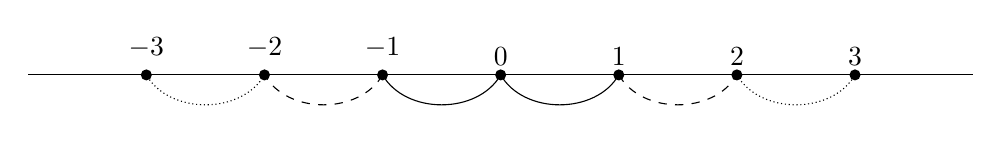
\begin{tikzpicture}[scale=1.5, every node/.style=fill,circle,minimum size=4pt,inner sep=0pt]
		\draw (0,0) to (8,0);
		\foreach \x in {1,...,7}
		{
			\node[label=above:{\pgfmathparse{\x - 4}% Evaluate the expression
				\pgfmathprintnumber[    % Print the result
				fixed,
				fixed zerofill,
				precision=0
				]{\pgfmathresult}}] at (\x,0) {};
		}
		
		\draw[bend angle=60,bend right] (4 ,0) to (5, 0);
		\draw[bend angle=60,bend left] (4,0) to (3, 0);
		
		\draw[bend angle=60,bend right, dashed] (4 + 1,0) to (5 + 1, 0);
		\draw[bend angle=60,bend left, dashed] (4 - 1,0) to (3 - 1, 0);
		
		\draw[bend angle=60,bend right, densely dotted] (4 + 2,0) to (5 + 2, 0);
		\draw[bend angle=60,bend left, densely dotted] (4 - 2,0) to (3 - 2, 0);
		
		\end{tikzpicture}
		\caption{Cutsets in $d=1$}
		\label{fig:7}
	\end{figure}
	Betrachten wir die Cutsets $\Pi_n$ wie in \autoref{fig:7}, so gilt 
	\begin{gather}
	(a \leftrightarrow \infty) \leq \sum\limits_{n \geq 1} \enb{\sum c(e) }^{-1} = \sum\limits_{n \geq 1 } \frac{1}{2} = \infty
	\end{gather}
	
	Sei $n = 2$, dann
	
	\begin{gather}
	\Pi_n = \set{e = (x,y) \given x \in Q_n, y \in Q_{n+1}}
	\end{gather}
	$Q_n$ sei der Quader der Kantenlänge $n$ \todo[inline]{missing figure}
	$\abs{\Pi_n} = 8n + 4$. Damit erhält man 
	\begin{gather}
	R(a\leftrightarrow \infty) \geq \sum\limits_{n \geq 1} \enb{\sum\limits_{c \in \Pi} 1}^{-1} = \sum\limits_{n \geq 1} \frac{1}{8n + 4} = \infty
	\end{gather}
	Nach Rayleigh (\ref{satz:Rayleigh}) genügt es für die Transienz den Fall $d=3$ zu betrachten. 
	
	\underline{Idee:} Wähle alle Pfade, die \enquote{direkt} von $0$ nach $\infty$ laufen \enquote{mit gleicher Wahrscheinlichkeit}.
	
	Wir wählen einen Punkt $s \in S^2$ nach dem Haarschen Maß. Konstruiere eine Gerade durch $\overrightarrow{0s}$. Wähle zu jeden $\overrightarrow{0s}$ einen Pfad in $\ZZ^3$, der nach $\infty$ läuft und \enquote{direkt} an $\overrightarrow{0s}$ liegt (Es gibt einen solchen Pfad, der Abstand $\leq 4$ hat). \todo{figuuuuure}
	Das gibt eine Menge von Pfaden $\set{(e_n)}$ und hierauf habe ich ein Wahrscheinlichkeit die durch das Haar--Maß induziert wird. Wir wollen für das wie in \eqref{eqn:4-1} konstruierte $\Theta$ $\mathcal{E}(\Theta)$ berechnen.
	\begin{align}
	\mathcal{E}(\Theta) &= \sum\limits_{e} \Theta^2(e) r(e) = \sum\limits_{e}\Theta^2(e) \leq \sum\limits_{e} \prop{e_n=e}[2] \\
	&= \sum\limits_{n=1}^{\infty} \sum\limits_{e\colon d(0,e^+) = n}\prop{e_n = e}[2] \\
	&= \sum\limits_{n = 1}^{\infty}Cn^2\frac{c'}{n^4} = const \sum\limits_{n \geq} \frac{1}{n^2} < \infty \marginnote{Es gibt $Cn^2$ viele Kanten mit $d(0,e^+) = n$} 
	\end{align}
	
	Die Wahrscheinlichkeit eine Kante zu benutzen ist nach oben beschränkt durch $\frac{c'}{n^2}$, weil durch die Wahl von $s$ alle kanten im Bastand \enquote{ungefähr gleich} häufig getroffen werden.
	
\end{beweis}



